%Document vide aux normes de l'École nationale des Chartes
%Dernières modifications E. Rouquette (12/2023)
	
	

\part{Partie 2 : Nouveaux catalogues, nouvelles interfaces, nouveaux usages}



%\setcounter{chapter}{0} % remet le compteur des chapitre à 1 

\chapter{Les interfaces : nouvelles architectures ?}
\begin{quote}
	\textit{2100, France, la Bibliothèque nationale vient d’achever la numérisation de l’entièreté de sa collection. Le site François Mitterrand, reflet de « l’utopie numérique »\footcite[p. 20]{bermes2024} de son fondateur à savoir numériser et rendre accessibles tous les savoirs conservés et qui devait être l’objet d’une réfection globale ne sera finalement pas restauré, mais transformé en habitations, jugé inutile. Le conservatoire d’Amiens suffisant à conserver l’entièreté du dépôt légal entrant, devenu entièrement dématérialisé. La consultation, seule vocation du site François-Mitterrand, ayant été déplacée en ligne, ce dernier n'a plus d'intérêt. La bibliothèque, en tant qu’emprise physique et Lieu de mémoire\footnote{En référence aux ouvrages parus sous la direction de Pierre Nora entre 1984 et 1992} n’est plus : remplacée par l’interface en ligne qui prend sa fonction symbolique, devant dès lors une architecture de pouvoir au sens propre ; volonté de la prestigieuse institution d’être le reflet de son histoire, nouveau Lieu de mémoire, elle concentre toutes les attentions.}
\end{quote}

Si évidemment cette uchronie est totalement fantasmée (cauchemardée ?) : il est inimaginable de voir les bibliothèques de consultation disparaître, elles qui mènent justement et avec brio des politiques centrées autour de l’accueil depuis des années. Il est tout aussi inimaginable de penser que le site François Mitterrand pourrait devenir inutile face à une société totalement digitalisée : le relatif échec des livres numériques en est la preuve. Il est de toute manière impensable que la numérisation de la totalité des collections de la Bibliothèque nationale de France soit un jour une réalité, cela n’aurait pas d’intérêt et serait coûteux (et encore, par rapport aux archives nationales, la Bibliothèque nationale de France numérise beaucoup). Mais il nous semblait intéressant de pousser à l’extrême un mouvement qui est bien réel : les interfaces prennent peu à peu, mais sans jamais les remplacer totalement, le rôle des lieux de consultation et deviennent, de fait, des \textit{Lieux de mémoire numériques }en tant que premier accès pour une immense partie des citoyens à la connaissance conservée. Elles se définissent comme la « jonction entre deux matériels ou logiciels leur permettant d’échanger des informations par l’adoption de règles communes physiques ou logiques »\footcite{zotero-205} c’est-à-dire qu’elles assurent la médiation de l’accès au savoir, dans le cas des institutions patrimoniales ; l’interface la plus courante est le catalogue. Cette question des interfaces prend donc une place centrale dans la découvrabilité des collections par leur rôle de médiation, et après avoir parcouru les enjeux autour de la notion de découvrabilité, il est intéressant de s’attarder sur ces dernières et d’analyser leur importance et leurs mutations récentes.

\chapter{« Vers de nouveaux catalogues »}

\vspace{-3em} % Réduit l'espacement vertical pour que la référence soit proche du titre.

\textit{En référence au titre d’un ouvrage paru en 2016 sous la direction d’Emmanuelle Bermès.}

\subsection{La transition bibliographique}

Pour parler de nouveaux catalogues et tenter de montrer comment et par quels moyens ils améliorent la découvrabilité des collections patrimoniales, il nous semble important de commencer par le début en abordant les raisons ainsi que l’historique de ces mutations. Cela nous permettra de tenter de distinguer les pratiques réellement nouvelles et novatrices des autres. Pour cela, nous commencerons par aborder la transition bibliographique que David Aymonin, directeur de l’Agence bibliographique de l’enseignement supérieur (Abes) présente ainsi : « On peut présenter la transition bibliographique simplement en expliquant que c’est une façon d’exprimer les métadonnées décrivant les documents sous forme d’entités et de relations. Cela fait presque 15 ans [en 2022, N.D.A] maintenant que les communautés de professionnels y travaillent, dans un monde de la documentation où tout est en transition. Nous avons le projet de partager les données de nos catalogues pour créer de nouveaux services […] il s’agit de créer des données riches, liées et accessibles à tous et sur lesquelles chacun peut s’appuyer pour les enrichir et développer de nouveaux services, de nouvelles activités, de nouvelles industries »\footcite[§3 et §4]{carre-marillonnet_transition_2022}. Ce programme a été mis en place conjointement par l’Abes et la Bibliothèque nationale de France et suit une logique mondiale impulsée par l’OCLC (la coopérative mondiale des bibliothèques).

Il s’appuie sur les principes de Paris, qui sont le cadre normatif du catalogage depuis 1961 avec en ligne de mire l’harmonisation des pratiques à l’échelle mondiale pour faciliter les échanges de notices et qui marquent la fin des catalogues sous forme de volumes papier et leur apparition sous forme de fiches catalographiques. Ces derniers ont été bouleversés en profondeur avec l’arrivée de l’informatique qui cassait la logique entre le contenu et sa forme matérielle (le livre en tant qu’unité intellectuelle étant confondu avec le codex, sa forme physique)\footcite[§ 2]{leresche_transition_2016} et posait le problème de la repérabilité des collections de bibliothèques décrites de façon peu adaptée aux logiques des moteurs de recherche\footcite[§ 2]{leresche_transition_2016}. Dans les années 1990, les limitations des Principes de Paris étaient donc importantes, c’est pourquoi l’IFLA (Fédération internationale des associations et institutions de bibliothèques) met en place un groupe de travail qui, plutôt que de remettre le livre en tant qu’unité intellectuelle au centre de sa réflexion, décide de poser la question de la modélisation de l’information bibliographique. En bref : qu’est-ce qu’un livre et qu’est-ce qu’une notice ? Le modèle FRBR (désormais renommé IFLA-LRM) est né. Comme nous l’avons déjà décrit dans notre partie 1, nous nous contenterons d’indiquer combien son approche est neuve pour les bibliothèques : désormais, c’est la notion d’entité qui est au centre du catalogue et l’importance est donnée à la structuration en réseau de ces dernières, suivant ainsi les principes du web en la matière (voir partie 1). Cela facilite aussi grandement les échanges entre les bibliothèques qui, en plus d’utiliser les mêmes formats (depuis les années 1970 et la mise en place du format MARC\footnote{Machine-Readable catalog}) peuvent désormais venir compléter leurs données avec celles des autres grâce aux standards du web tout en résolvant les problèmes posés par les principes de Paris. Notamment la difficulté à décrire une œuvre matérialisée dans différentes expressions ; cela répond par ailleurs mieux aux demandes des utilisateurs qui privilégient l’information « brute » à une liste d’ouvrages quand ils font une recherche\footcite[§ 13]{leresche_transition_2016}. Toutes ces mutations, regroupées sous le nom de transition bibliographique, ont permis l’émergence de portails et des échanges de données plus importants (ainsi que la mise en place d’initiatives telles que data.bnf.fr décrit plus haut) qui seront l’objet de notre prochaine partie.

\subsection{Les portails et le moissonnage des données}



Nous avons évoqué dans notre première partie que l’un des enjeux derrière le projet data.bnf.fr et le web sémantique de manière plus générale, outre le fait de sortir les données des bibliothèques du web profond, était de « casser les silos ». C’est-à-dire de passer outre la matérialité documentaire pour venir la dépasser. Car comme évoqué par Emmanuelle Bermès dans son article « Vers un catalogue orienté entités : la FRBRisation des catalogues »\footcite{bermes_vers_2016}, ce qui intéresse les utilisateurs, ce ne sont pas les livres, mais bien l’information qu’ils contiennent, la structuration des catalogues en tant que « listes de livres » n’étant que l’illustration de la contrainte physique qu’ils imposaient avant l’arrivée de l’informatisation en bibliothèque\footcite[§ 2]{bermes_vers_2016}. Ces derniers ne l’ont d’ailleurs pas totalement attendue pour tenter de dépasser cette limitation, notamment en proposant différents points d’entrée (auteurs, classification, etc.) vers leurs collections au moyen de fiches catalographiques\footcite[§ 5]{bermes_vers_2016}.

En passant du concept de documents à celui d’informations, les institutions patrimoniales, bibliothèques en tête, viennent casser les frontières : un utilisateur qui fera une recherche sur Exékias, peintre et potier athénien, se verra ainsi proposer en un seul et même point toutes les informations sur ce dernier : sa biographie sur Wikipédia, la liste de ses œuvres conservées au Louvre, la liste des ouvrages et articles qui lui ont été consacrés sur le catalogue général de la BnF… On sort ici du concept de catalogue « Énumération précise, méthodique, exhaustive des éléments d’une collection »\footcite{zotero-197} pour glisser vers celui de portail « site web qui offre une porte d’entrée commune à un large éventail de ressources et de services accessibles sur Internet »\footcite{2024} où la notion centrale est celle de ressources.

De façon plus technique, au centre de la notion de portails est celle de moissonnage qu’il nous faut décrire ici. Pour ce faire, nous prendrons l’exemple du protocole OAI-PMH (pour Open access initiative, protocol metadata harvesting) qui reste très utilisé (notamment dans Gallica et Europeana) même s’il a tendance à être dépassé par d’autres. Créé à la fin des années 1990 par des institutions désireuses d’échanger leurs métadonnées descriptives, ce protocole « définit comment un site web peut exposer des métadonnées et permettre leur récupération par tout client intéressé »\footcite[§ 22]{mesguich_5_2017}. Le moissonnage correspond à la récupération par le client. Pour que ce dernier soit effectif, il est essentiel que les données suivent un format normalisé. Par exemple, si je souhaite récupérer la liste des œuvres d’Exékias, si le Louvre structure ses données ainsi : \texttt{<listOeuvres> Coupe à figure rouge n° 512, Amphore à figure noires n° 518 </listOeuvres>} alors que le petit Palais les structure ainsi : \texttt{<œuvres> Cratère à figure noires, œnochoé à figures rouges </œuvres>}, même si les deux musées décrivent la même chose, l’éventuel portail (client) qui viendrait moissonner les sites de ces deux musées serait incapable de comprendre qu’il s’agit des mêmes données exprimées avec des noms différents. Ainsi, au cœur de la mise en place de portails se trouve la notion de données dites « FAIR », c’est-à-dire : facilement trouvables, accessibles, interopérables, réutilisables. Qui, comme son nom ne l’indique pas, se situe plutôt du côté des choix institutionnels que des données : pour qu’elles soient FAIR, il faut avant tout un choix politique fort de la part des institutions, qui sera ensuite traduit en choix techniques.

C’est ce qu’illustre très bien la mise en place du cadre d’interopérabilité IIIF (International image interoperability framework) au sein du portail France Archives déjà évoqué. Comme son nom l’indique, IIIF ce sont un ensemble de normes techniques (utilisation du format JSON et d’une syntaxe normée notamment) pour décrire et accéder à des images sur le web par le biais de visionneuses spécifiques. Outre le fait qu’exposer des données en suivant les normes et recommandations techniques de la communauté IIIF améliore le référencement des images en permettant aux moteurs de recherche de mieux les indexer, cela permet aussi de les mettre à disposition de façon standardisée pour les utilisateurs (privés ou institutionnels) afin qu’ils puissent les modifier, les annoter ou simplement les afficher dans des interfaces de consultation (visionneuses) standardisées (par exemple \url{https://projectmirador.org/})\footcite{robineau_programme_2023}. À l’échelle des institutions, la mise en place de IIIF peut permettre de créer des portails de consultations communs et fédérés et donc de mutualiser les moyens bien sûr, mais aussi les collections. Par exemple, aux archives départementales du Lot-et-Garonne, un projet est en cours pour mettre en ligne, en suivant les principes de IIIF, le fonds Lauzun, du nom d’un érudit local ayant rassemblé des clichés archéologiques au cours du XIXe siècle afin que les images soient moissonnées par le portail France Archives. Outre tous les avantages déjà décrits plus haut, il faut noter qu’une partie de ce fonds est conservée par les archives départementales du Gers voisines ; le mettre à disposition dans un portail permettrait donc — si les archives départementales du Gers suivent le choix de celles du Lot-et-Garonne — de rassembler virtuellement un fonds qui a une unité intellectuelle, mais pas physique\footcite{brunet_archives_2023}. Mais c’est bien parce que les archives départementales du Lot-et-Garonne ont fait le choix institutionnel de mettre leurs images numérisées à disposition de façon ouverte, en suivant un format interopérable pour favoriser leur réutilisation, que ces dernières se retrouvent accessibles et rayonnent à l’échelle nationale au travers de France Archives, portail français des archives. Cela permet donc aux utilisateurs cherchant une information de la trouver, sans égard pour le lieu qui la conserve, améliorant ainsi la repérabilité de cette dernière ainsi que son référencement : être sur un portail national, voire européen, peut faire sortir du web profond des collections qui n’en auraient, autrement, pas forcément eu les moyens techniques. Cela pose en revanche la question de l’invisibilisation des institutions qui ne deviennent que des puits de données, et c’est l’une des limites de ce type de pratique (car les financements vont aux établissements les plus visibles bien souvent).

\subsection{Des catalogues aux politiques \textit{data driven}}

Et si les données, plutôt que d’être vues comme de vastes réservoirs parfois difficiles à gérer, étaient abordées comme un moyen d’être plus efficace ? Et si l’amélioration de leur découvrabilité rendait des services, non seulement aux usagers externes (dans le cadre patrimonial), mais aussi en interne ? Car l’exponentielle augmentation de la masse des données disponibles est aussi accompagnée d’une grande diversification de ces dernières, et le secteur patrimonial ne fait pas ici exception\footcite[§15 à §18]{poupeau_donnee_2016}. Ces dernières peuvent aller des métadonnées catalographiques classiques aux traces laissées par les usagers en ligne en passant par les données juridiques. On a vu plus haut combien les projets de portails permettaient de casser les silos de données, améliorant, de fait, la découvrabilité, mais seuls les silos documentaires sont ici brisés. Reste ceux internes aux institutions, en liant toutes les données entre elles, les institutions peuvent optimiser leur processus, et notamment documentaires. C’est par exemple le cas à la RTS, après le lancement de GICO\footnote{L'outil de gestion des données archivées par la RTS déjà évoqué dans la partie 1}. La volonté a été d’y intégrer des données juridiques, l’idée attenante était de permettre aux documentalistes de voir, directement lors de leur recherche, quelles images étaient encore sous droits et quelles images étaient propriété de la RTS. Même si le projet a été au final abandonné, du fait de sa complexité et de problématiques internes, qu’il serait fastidieux de détailler ici\footcite{barcella2024a}, l’idée était présente : casser les silos internes pour permettre une gestion plus efficace de l’information.

Comme l’écrit Gauthier Poupeau dans « La donnée : nouvelle perspective pour les bibliothèques »\footcite{poupeau_donnee_2016} il s’agit pour les bibliothèques et institutions patrimoniales de manière générale « d’arrêter de faire du catalogue le centre de leur système d’information » et « de faciliter l’accès aux documents par l’utilisation de nouvelles données issues de l’exploitation du contenu lui-même et de l’analyse des traces laissées par les utilisateurs »\footcite[§ 3]{poupeau_donnee_2016}. C’est exactement cette démarche qui a été entreprise par l’Institut national de l’audiovisuel (INA), qui a mis en production un lac de données en 2022 pour répondre aux problématiques énoncées plus haut. Car les données de l’institut fondé en 1974 après l’éclatement de l’Office pour la radiotélévision française (ORTF) sont elles aussi très diverses : dépôt légal des flux télévisuels et radiophoniques (depuis 1995), d’une partie du web, base juridique, référentiels, données de production, traces, métadonnées moissonnées depuis diverses sources (Médiamétrie par exemple), bases commerciales…\footcite{alquier2024} Ce lac a eu pour vocation de briser les silos entre deux systèmes d’information très opaques entre eux : le dépôt légal et les métadonnées patrimoniales d’une part et de l’autre le système dit « professionnel »\footcite[p. 195]{dribault_dujardin_levolution_2020}. Le modèle de données (manière dont les données sont organisées) se veut le plus simple possible avec à son origine un événement, par exemple la diffusion de « Quand les dieux rôdaient sur la terre » à la radio auquel on peut ajouter tout type de données : l’émission en tant que telle et ses métadonnées, le post Instagram réalisé pour en faire la promotion, ou encore une — hypothétique — captation vidéo de l’émission. Le tout, dans l’objectif d’être le plus souple possible et de répondre aux évolutions actuelles et futures de l’univers médiatique et de son archivage bien sûr, mais aussi des technologies et des besoins des utilisateurs ainsi que des apports externes (notamment concernant les métadonnées) qui sont nombreux au sein de l’institution\footcite[p. 198]{dribault_dujardin_levolution_2020}. Cela permet à l’INA d’avoir à disposition, plus qu’un lac, un véritable océan de données constitué de 5 milliards de lignes\footcite{alquier2024} de description dans lequel les usagers et les outils peuvent puiser à volonté, garantissant une gestion bien plus efficace et normée. Ainsi, chercheurs, commerciaux, documentalistes peuvent exploiter les données pour répondre à leurs besoins, et c’est exactement ce que fait l’Institut avec la mise en place d’outils de traitement des images par exemple qui viennent encore alimenter le lac.


\begin{figure}[h!]
	\centering
	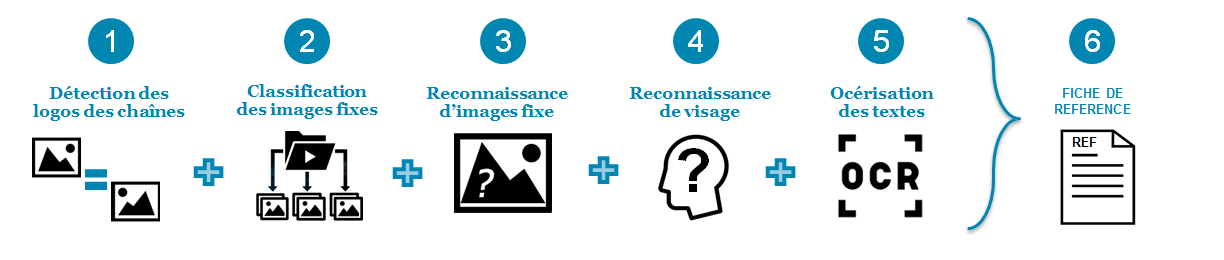
\includegraphics[width=0.8\textwidth]{images/image11.png}
	\caption{Traitements effectués par l'INA sur une image}
	\label{fig:image11}
\end{figure}


\begin{center}
	Depuis \enquote{L'évolution des pratiques de description des archives documentaires...} page 199. 
\end{center}

L’institution a aussi la possibilité d'utiliser les données ainsi organisées pour réaliser des visualisations de données, avoir pris le temps de les structurer rend en effet bien plus aisées et pertinentes ce type de réalisations. En témoigne le projet Data.INA.fr (qui sera évoqué dans notre troisième partie). Les visualisation de données seront ainsi l’objet de notre prochaine partie en tant que nouveau type d'interfaces d'accès au savoir.

\chapter{La visualisation de données en tant que nouvelle interface au service de la découvrabilité}

\subsection{Voir globallement : l'importance d'avoir une vue d'ensemble des collections}


Comme décrit plus haut, la digitalisation du patrimoine a créé des volumes de données immenses et a, dans le même temps, changé notre rapport au patrimoine qui est devenu plus intangible\footcite[p. 1]{windhager_visualization_2019}, plus « virtuel ». Aux salles de lecture d’archives saturées des années 1980, ont succédé des sites web qui le sont tout aussi — si ce n’est plus. Dans le cas du patrimoine audiovisuel, massivement numérisé dans les années 2000 comme décrit, les interfaces sont très souvent les seuls moyens d’accéder aux objets patrimoniaux. Cette nouvelle approche d’un patrimoine intangible, accessible par le biais d’interfaces web basées sur les métadonnées, change les pratiques et usages, notamment le sens de recherche : là où les chercheurs démarraient aux niveaux hiérarchiques hauts (fonds, collections, etc.), les moteurs de recherche donnent aujourd’hui accès au niveau de la pièce directement, rendant difficile l’appréhension des collections dans leur ensemble et rejoignant le concept déjà de « fatigue muséale »\footcite[pp. 62-72]{gilman_museum_1916}. Les interfaces web classiques : une barre de recherche et des filtres à facettes viennent reproduire, et même amplifier, cette problématique de fatigue muséale ; les utilisateurs occasionnels étant souvent confrontés à un syndrome de la barre de recherche blanche. Sans vue d’ensemble sur les fonds, ils ne sont pas capables d’aller les explorer. C’est pourquoi, le concept d’interfaces dites généreuses est né\footcite[pp. 5-6]{windhager_orchestrating_2018}, elles partent du postulat que l’utilisateur n’est plus un chercheur en manque d’information, mais un flâneur qui souhaite découvrir le fonds. La priorité de telles interfaces, contrairement aux barres de recherche qui favorisent la « trouvabilité », est de favoriser la découvrabilité\footcite[p. 18]{shen_generous_2023}. La visualisation de l’information (ou \textit{data visualization}) prend alors une importance nouvelle puisqu’elle peut permettre de réduire cette fatigue muséale tout en améliorant la découvrabilité des fonds.

Prenons ici comme exemple l’expérience conduite par le laboratoire de recherche de la bibliothèque publique de New York « le catalogue en réseau »\footcite[§20 à §26]{lapotre_visualiser_2016}, dont l’objectif était de montrer la totalité du catalogue sur une seule image et de voir les relations qu’entretiennent les objets entre eux, comme si le catalogue avait un bouton « voir tout »\footcite{miller_networked_2014}.


\begin{figure}[h!]
	\centering
	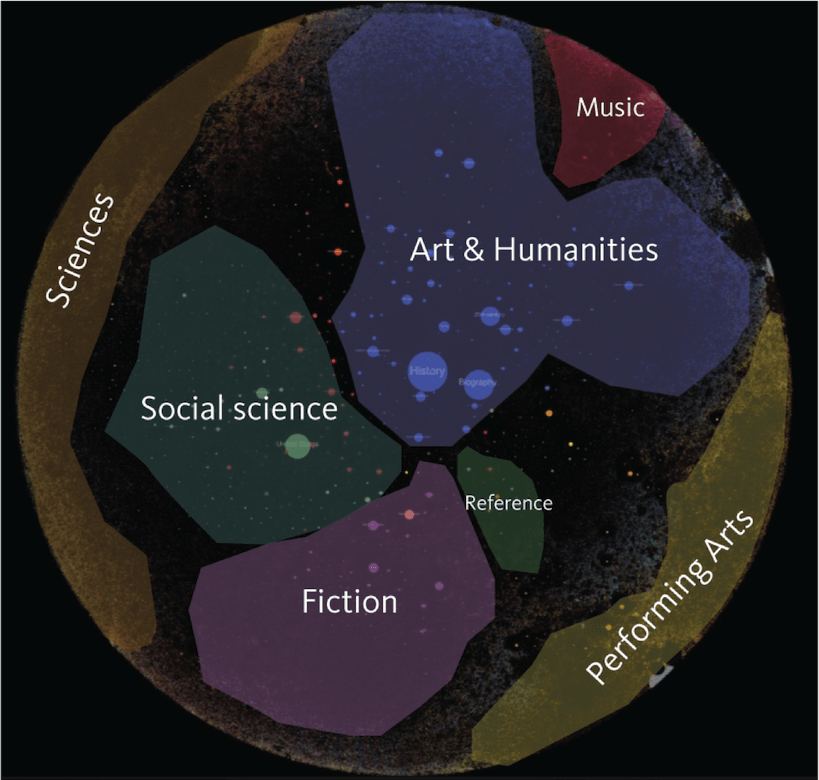
\includegraphics[width=0.8\textwidth]{images/image12.png}
	\caption{Illustration des grandes thématiques se dégageant de l'expérimentation de la bibliothèque publique de New York}
	\label{fig:image12}
\end{figure}

\begin{center}
	Depuis \enquote{The networked catalog}, Miller...
\end{center}


Techniquement parlant, cette visualisation utilise les descripteurs \textit{MARC} d’indexation de chaque item et les affiche sous forme de points colorés : plus un point est gros, plus il y a d’ouvrages le concernant dans la bibliothèque publique de New York ; si deux sujets sont souvent mentionnés ensemble, par exemple Jeux-Olympiques et sport, on en déduit qu’ils sont liés d’une manière ou d’une autre et ils se voient attribuer la même couleur.

Outre le fait qu’elle soit fascinante et que l’explorer et s’y perdre soit passionnant\footnote{La navigation interactive est disponible en suivant ce lien : \url{ http://catalog-network.s3-website-us-east-1.amazonaws.com/}}, elle permet, d’un coup d’œil, de se rendre compte des pans de la collection très représentés et centraux ainsi que des liens sémantiques, parfois étonnants entre des entités. Cela permet de se rendre compte de ce qu’une bibliothèque, en tant que réceptacle du savoir à un instant donné, conserve le plus. La visualisation peut donc être, comme l’écrit Raphaëlle Lapôtre, « un moyen heuristique qui participerait à la production de connaissances »\footcite[§ 23]{lapotre_visualiser_2016}. En plus de donner une vision d’ensemble et de favoriser la compréhension globale de la collection, elle permet de lui faire dire de nouvelles choses. On serait évidemment tenté de voir dans cette image une visualisation des connaissances, comme si une bibliothèque était le reflet du réel et des connaissances produites, mais il est déformé : parce que le contenu d’une bibliothèque (hors dépôt légal) est le reflet des politiques documentaires de son époque ; parce que les données ne sont pas si fiables, qu’elles sont truffées d’erreurs humaines ; de choix d’indexation ; des migrations de données et des changements de vocabulaires. Par exemple, le mot tsunami n’est employé que depuis récemment, on lui a longtemps préféré « raz de marée »\footnote{Propos rapportés par Denise Barcella}.

Éclairons notre propos avec l’exemple de la RTS où l’on a voulu effectuer une démarche similaire pour proposer un outil de navigation sous forme de \textit{treemap} hiérarchique en utilisant les codes contenus, métadonnées fournies pour chaque document renseignant sa thématique de façon hiérarchique, par exemple un téléjournal sera classé sous actualité.



\begin{figure}[h!]
	\centering
	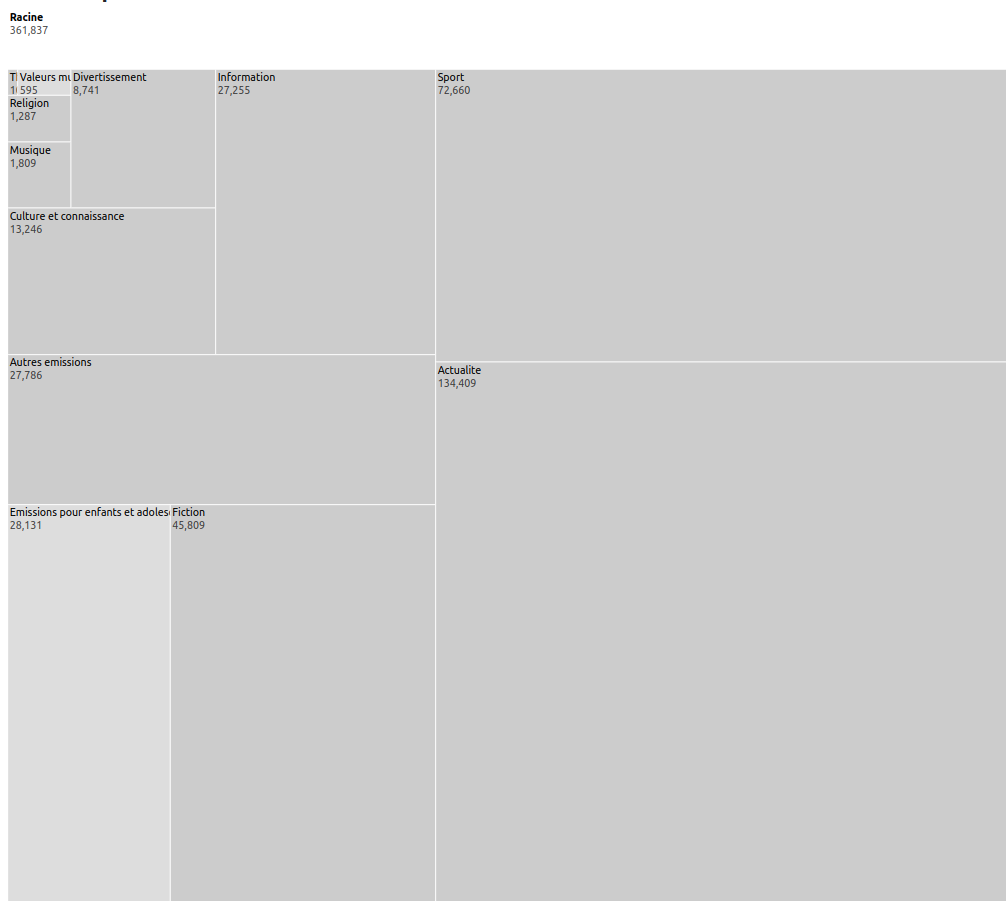
\includegraphics[width=0.8\textwidth]{images/image13.png}
	\caption{Treemap interactive réalisée pendant le stage}
	\label{fig:image13}
\end{figure}



Une fois la visualisation réalisée, nous nous sommes rendu compte qu’elle n’était absolument pas le reflet de ce qui était conservé à la RTS. D’abord, car seule une petite proportion des documents avait un code contenu renseigné (361 837 documents), ensuite car ce qui fait varier la taille des rectangles, le nombre d’items, ne reflète pas la réalité : il n’y a pas plus de sport que de fiction diffusée, c’est simplement qu’on conserve et indexe rarement la fiction qui est souvent achetée en externe. Par ailleurs, on retrouve énormément d’actualité, ce qui est en partie vrai, mais elle est aussi beaucoup représentée, car c’est la seule, depuis les années 1980, à être archivée de façon systématique. Comme la carte de la bibliothèque publique de New York était plus le reflet de son histoire institutionnelle et documentaire, cette visualisation est le reflet des pratiques documentaires de la RTS plus que de ce qui est conservé en son sein. Dans les deux cas, surtout à New York, l'objectif de donner une vision d'ensemble de la collection semble accompli. Les possibilités heuristiques offertes par la visualisation de données, une fois les spécificités et biais potentiels pris en compte, sont prometteuses. En effet, cela permet d'envisager de fournir aux utilisateurs des collections des clés de lecture différentes, qui feront l'objet de notre prochaine partie.

\subsection{Voir sous un autre angle : donner des clés de lecture différentes des collections}

On vient de voir que la visualisation de l’information, en plus d’offrir une indispensable vue d’ensemble des collections, offre un potentiel heuristique nouveau. Elle permet en effet « d’opérer un “point de vue” sur un sous-ensemble de résultats pertinents afin d’en faciliter la compréhension »\footcite[§ 3]{hachour_fouille_2015} ; l’intérêt de visualiser des données est donc d’offrir aux regardeurs différentes clés de lecture\footnote{ « Concept ou angle d’approche permettant de comprendre, d’analyser, d’interpréter ou encore de critiquer un texte, une œuvre, ou un phénomène. » - Wikictionnaire } d’une collection. On peut séparer ces clés de lecture en trois catégories (qui peuvent se cumuler) : vues multiples (listes, mosaïques, etc.) ; encodage spatial (cartes géographiques, diagrammes de réseau, etc.) et encodage temporel (frises chronologiques, animations)\footcite[p. 76]{windhager_review_nodate}. À chaque catégorie correspondent des possibilités interprétatives différentes, par exemple : un diagramme en réseau permet d’explorer la proximité entre des objets culturels, une animation temporelle permet de donner à voir les évolutions temporelles des objets\footcite[p. 77]{windhager_review_nodate}.

La multiplication des interfaces de visualisation offre aux utilisateurs un accès riche et non restrictif aux collections culturelles, ce qui permet d’explorer des ensembles de données vastes. Ce faisant, ces différentes interfaces sont des outils précieux pour exposer la richesse et la diversité des collections culturelles afin que les utilisateurs puissent naviguer entre différentes perspectives. Pour les qualifier, F. Windhager et al. parlent d’« interfaces généreuses ».\footcite[p. 5]{windhager_orchestrating_2018} qui se distinguent des interfaces classiques par une capacité à présenter de grandes quantités d’informations en soutenant les utilisateurs dans leurs tâches cognitives afin de limiter la fatigue. De même qu’un bâtiment doit être généreux et offrir des espaces vides et des plafonds hauts pour être agréable à utiliser, les interfaces, en tant que substituts théoriques, doivent faire de même.

Elles doivent donc être conçues pour éviter la surcharge cognitive en offrant des représentations multiples des données, ce qui permet aux utilisateurs de construire une vision globale et cohérente des collections qu’ils explorent\footcite[pp. 5-6]{windhager_orchestrating_2018}. Elles se veulent des « anti barres de recherche », car, selon les auteurs, ces dernières sont construites selon deux suppositions préalables : le visiteur connait, au moins vaguement, ce qu’il cherche et il ne souhaite pas « s’engager dans la complexité de l’espace de recherche qui leur est caché »\footcite[p. 6]{windhager_orchestrating_2018}.

Afin d’illustrer notre propos, nous mettrons en parallèle un exemple issu d’une réalisation pendant le stage (carte interactive des contenus archivés par la RTS) et le tableau de bord réalisé par la Bibliothèque du Congrès pour visualiser la presse numérisée\footcite[tableau de bord accessible en suivant l'url suivante \url{https://public.tableau.com/app/profile/chronicling.america/viz/ChroniclingAmericaTemporalCoveragebyStateMap/TemporalStateCoverage}]{noauthor_chronicling_nodate}.

D’abord, donc, la carte interactive des contenus qui se présente, comme son nom l’indique, sous forme d’une carte de la Suisse avec la possibilité de naviguer entre les différents niveaux territoriaux du pays : cantons, districts et communes. Elle permet, en un seul regard, d’observer les territoires pour lesquels la RTS conserve le plus d’archives et de cliquer sur ces derniers pour consulter les archives qui s’y réfèrent. Elle combine les niveaux de lecture spatiaux et temporels décrits plus haut en permettant aux utilisateurs de naviguer dans le temps pour observer les variations dans la collection. Par ailleurs, ils ont la possibilité d’inclure un terme de recherche pour observer la répartition géographique de ce terme. Par exemple, dans l’image ci-après, on a tapé « abricots » et on observe que le canton le plus représenté est le Valais\footnote{Canton produisant 90 \% des abricots Helvètes}. Cette carte n’est donc pas uniquement un outil d’exploration, elle permet aussi de réaliser des statistiques à partir des recherches effectuées en proposant un export (au format Excel) de ce qui est visualisé.



\begin{figure}[h!]
	\centering
	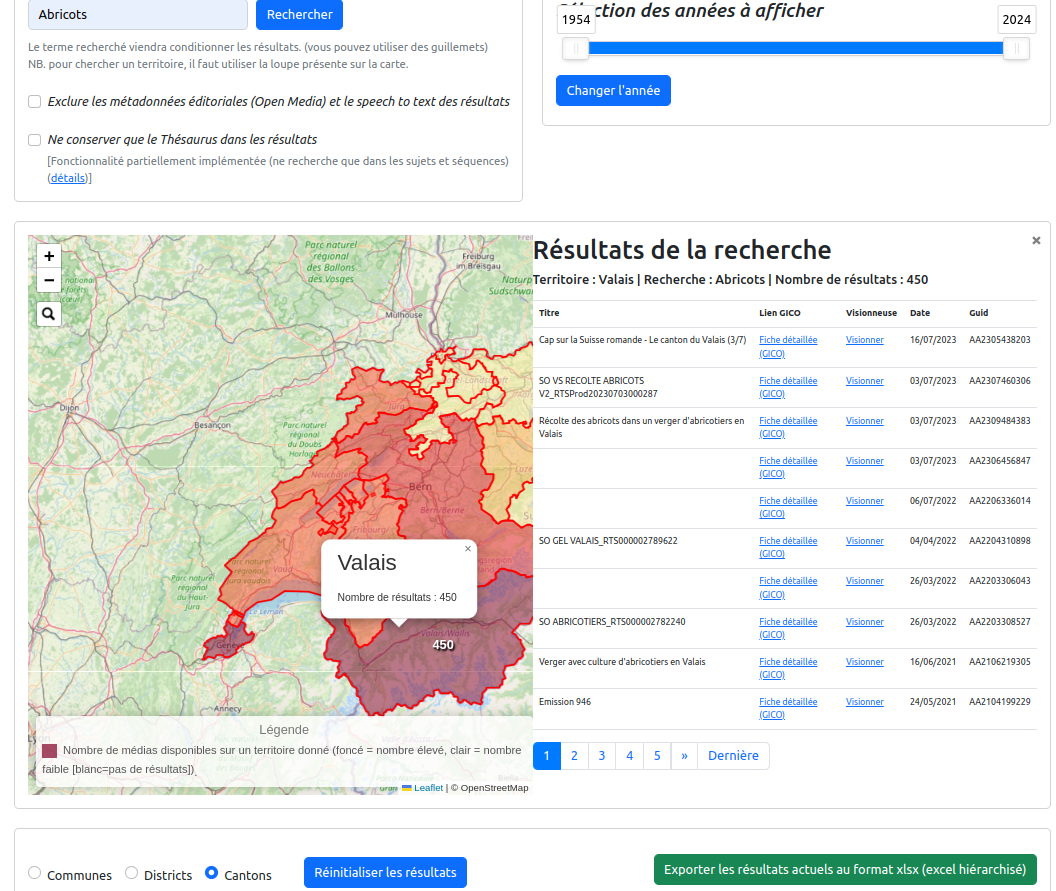
\includegraphics[width=0.6\textwidth]{images/image14.png}
	\caption{Carte interactive des contenus archivée à la RTS réalisée pendant le stage}
	\label{fig:image14}
\end{figure}


Ensuite, le tableau de bord de la Bibliothèque du Congrès, ce dernier est aussi interactif et propose aux utilisateurs de voir le nombre de journaux numérisés disponibles dans chaque État. C’est là aussi une interface qui combine une lecture spatiale et temporelle, mais, ici, le choix a été fait de séparer ces deux clés de lecture, la carte permet de sélectionner l’État pour que l’utilisateur puisse visionner le nombre de titres de presse disponibles et numérisés à travers le temps. Cette interface ne permet, en revanche, pas de consulter directement les titres de presse.


\begin{figure}[h!]
	\centering
	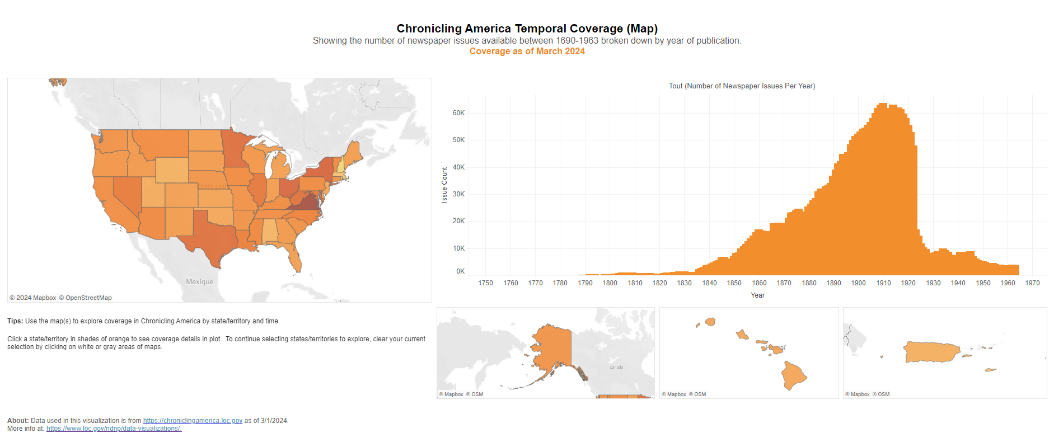
\includegraphics[width=0.8\textwidth]{images/image15.png}
	\caption{Tableau de bord \enquote{Chronicling America Maps and Visualizations}}
	\label{fig:image15}
\end{figure}


On a donc ici deux approches similaires, mais avec des visées différentes, la première approche est plus du côté de l’interface de navigation dans les collections, la seconde est statistique. Dans les deux cas, on offre aux utilisateurs la possibilité de voir dans son ensemble un fonds extrêmement volumineux en proposant des clés de lecture variées. Soit elles sont combinées dans une seule visualisation à l’aide de filtres, soit elles sont séparées en deux visualisations différentes. Cette vision d'ensemble permet aux personnes consultant les fonds de ne pas tomber dans certains écueils. Par exemple, dans le cas de la RTS, étant une chaîne romande, la majorité des sujets concerne la région linguistique francophone. Si l'on souhaite effectuer une recherche sur des cantons italophones ou germanophones, ce ne sera pas l'endroit le plus pertinent. Ce type d’interface répond donc à de multiples problématiques : donner une vision d’ensemble et des clés de lecture différentes d’un fonds ; permettre une interprétation quantitative ; être utilisé dans des actions de valorisation tout en limitant le syndrome de la barre de recherche blanche décrit plus haut. Par ailleurs, la multiplicité des filtres permet une granularité de navigation très importante donnant de nombreuses opportunités de se concentrer sur des documents spécifiques\footcite[p. 7]{windhager2018a}. Combiner différentes clés de lecture (dans le cas de la RTS, nous avons ajouté à cette visualisation un \textit{knowledge graph} visible plus bas) en prenant en compte le fait que chacune permet de capturer un aspect spécifique de la collection est donc une stratégie intéressante dans le cadre d’objets culturels complexes. Par ailleurs, cela permet de créer des possibilités pour les utilisateurs de faire des découvertes par sérendipité, car ce type d’interface les laisse « flâner » dans les collections comme le notent Thudt et al.\footcite[(cité dans)]{windhager2018a}. En revanche, comme le notent Florian Windhager et al., réaliser des interfaces généreuses combinant de nombreuses visualisations et possibilités de filtrage peut recréer la problématique de fatigue muséale citée plus haut en créant ce que les auteurs appellent le « split attention challenge »\footcite[p. 9]{windhager2018a}. Les interfaces, de même que les bâtiments, doivent donc, tout en restant généreuses, ne pas proposer trop de niveaux de lecture et rester simples d’utilisation, car dans les deux cas, cela résulte en un usager perdu : dans l’immensité de l’espace physique ou virtuel (ici aussi, le site François Mitterrand est éclairant).

\begin{figure}[h!]
	\centering
	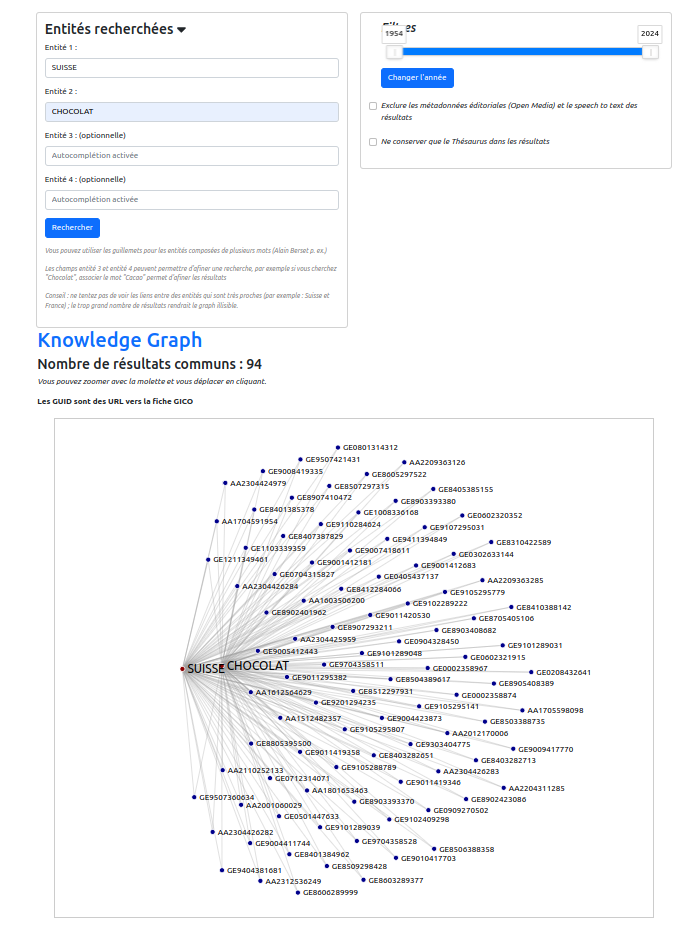
\includegraphics[width=0.8\textwidth]{images/imageknowledge.png}
	\caption{\textit{Knowledge Graph} réalisé pendant le stage}
	\label{fig:imageknowledge}
\end{figure}


\subsection{Voir pour aller plus loin}

Dans la partie précédente, nous avons montré que les interfaces pouvaient permettre de se substituer aux bâtiments en proposant une vue d’ensemble des collections et une navigation dans cette dernière, à la manière des déambulations dans un lieu physique. Mais les interfaces peuvent-elles permettre d’aller plus loin ? Peuvent-elles permettre de dépasser les capacités humaines en matière de découvrabilité ? Pour tenter de répondre à ces questions, nous allons explorer le projet de recherche Philherit présenté lors de la journée d’étude organisée par la Bibliothèque nationale de France le 20 juin 2023 « penser la découvrabilité des contenus culturels »\footcite{plouviez_philosophie_2023} et le projet \textit{Impresso} (projet d’exploration de corpus de la presse écrite [images et textes])\footcite{noauthor_impresso_nodate}.

Comment poser la question de l’héritage dans le domaine de la philosophie de nouveau ? C’est la question que pose le projet Philherit. Pour y répondre, le corpus à analyser est extrêmement vaste, car la question était centrale au XIXe siècle\footcite{plouviez2023} du fait de sa proximité avec les questions de justice sociale entre autres. Ce corpus se constitue, par ailleurs, de sources très variées (périodiques, livres, journaux, etc.) et dans toutes les disciplines (économie, philosophie, etc.) réparties en sept bases de données textuelles extraites depuis Gallica. Le texte est ensuite réparti en différents thèmes identifiés par trois mots-clés grâce à l’intelligence artificielle (\textit{BERT})\footnote{En traitement automatique du langage naturel, BERT, acronyme anglais de Bidirectional Encoder Representations from Transformers, est un modèle de langage développé par Google en 2018 - Wikipédia}. Ce qui est intéressant ici, pour revenir à la question des interfaces, c’est la mise en place d’un nuage de mots qui reprend les thèmes générés par l’intelligence artificielle et les donne à voir de façon synthétique : plus un mot sera gros, plus il sera représenté dans le corpus, ce qui permet de dégager de grands thèmes et d’aller consulter les ouvrages essentiels\footnote{Il nous a été impossible de trouver une image de bonne qualité de cette interface, elle est tout de même visible dans la vidéo suivante : \url{https://youtu.be/4zaebvULdc4?t=4787} à 1h19 et 47 secondes.}. Mélanie Plouviez, dans son intervention, dégage trois impacts de l’utilisation des interfaces pour l’amélioration de la découvrabilité du corpus : premièrement, l’accélération de l’analyse, qui était avant réalisée sur \textit{Excel} manuellement et est désormais possible d’un seul coup d’œil sur l’interface ; deuxièmement, l’amélioration de l’analyse dite « hypertextuelle », c’est-à-dire de l’exploration des liens entre les documents ; et, troisièmement, l’amélioration de la sérendipité\footcite{plouviez2023}. La chercheuse conclut son intervention en citant Michel Foucault qui, dans son \enquote{archéologie du savoir}\footcite{foucault_archeologie_2008}, définissait les archives comme une « masse discursive » à laquelle les humanités numériques auraient mis fin tout en permettant de faire émerger de multiples points de vue d’une même masse documentaire grâce aux multiples possibilités d’interfaces\footcite{plouviez_philosophie_2023}.

Les interfaces permettent-elles de dépasser les capacités humaines uniquement dans le cadre de projets spécifiques et de cas d’usages précis ? Attardons-nous sur le projet \textit{Impresso}, dont l’objectif est d’améliorer la découvrabilité de la presse numérisée suisse et luxembourgeoise (donc en 4 langues). Il est mené par une équipe interdisciplinaire d’historiens, linguistes et informaticiens ainsi que des designers — essentiels pour la réalisation d’interfaces efficaces\footcite{ehrmann_explorer_2021}. Ici, en plus de répondre à des cas d’usages « de chercheurs », le projet tente d’être accessible et utile pour les non-spécialistes en répondant à cinq cas d’usages : récupération du contenu utile, compréhension et contextualisation, comparaison des résultats, exportation pour analyse et transparence (documentation du code) et explicabilité de ce dernier\footcite[pp. 5-7]{during_transparent_2024}. L’interface répond donc à ces cas d’usages en offrant, entre autres choses\footnote{Nous ne décirons pas ici toutes les fonctionnalités, ce serait trop fastidieux.}, la possibilité pour ses utilisateurs, une fois un terme recherché, de compléter leur recherche. Soit de façon thématique, avec des personnalités liées, ou bien des collections liées ; sans tenir compte de la langue de leur recherche.

\begin{figure}[h!]
	\centering
	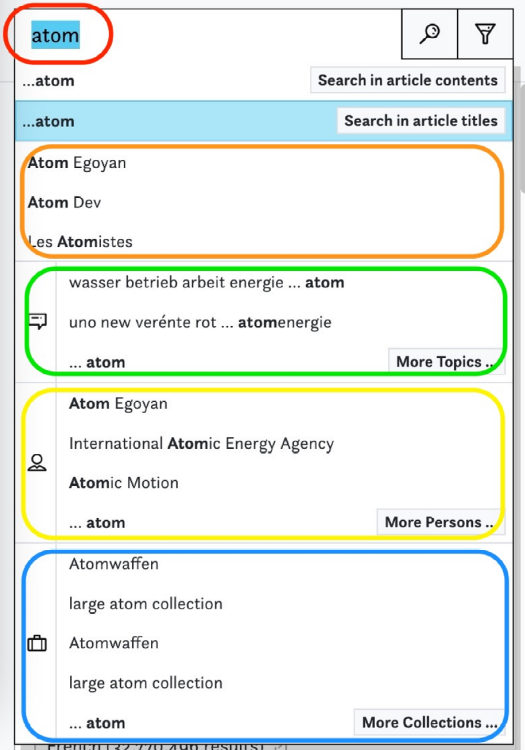
\includegraphics[width=0.3\textwidth]{images/image16.png}
	\caption{Illustration de l'autocomplétion des recherches, depuis \textit{Düring, Bunout, Guido...}}
	\label{fig:image16}
\end{figure}
\newpage

Elle permet aussi de voir les textes et images similaires pour un sujet donné et de voir sa distribution dans le temps en suivant le principe des \textit{n-grams}\footnote{ Un n-gramme est une sous-séquence de n éléments construite à partir d'une séquence donnée - Wikipédia. }. Enfin, elle permet de comparer différents résultats pour observer leur traitement dans la presse. Par exemple, on peut choisir d’observer les résultats communs entre « abricots » et « Valais », et on se rendra compte que l’année du pic observé (1953) correspond à la « révolte des abricots »\footcite{noauthor_revolte_2018}.

\begin{figure}[h!]
	\centering
	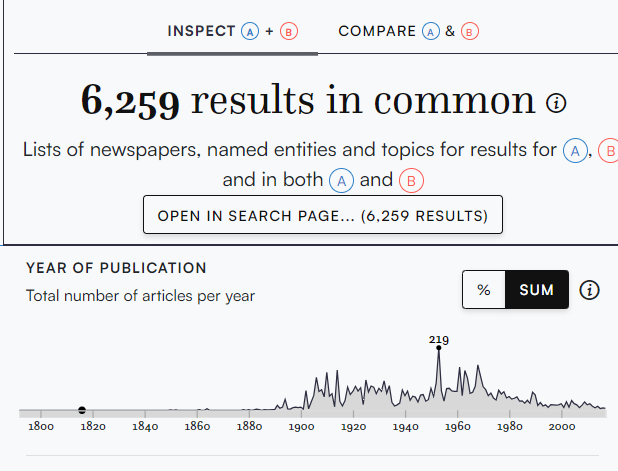
\includegraphics[width=0.6\textwidth]{images/image17.png}
	\caption{Recherche comparative entre \enquote{abricots} et \enquote{Valais}}
	\label{fig:image17}
\end{figure}

Il semble, à en lire les évaluations des utilisateurs, que les fonctionnalités proposées et l’interface soient non seulement faciles d’accès, mais permettent en outre une grande finesse dans l’exploitation de ce type de corpus textuel. Par ailleurs, les auteurs concluent en énonçant le fait que les chercheurs déjà habitués aux recherches « \textit{data-driven} » étaient très positifs sur les possibilités d’export et d’exploitation offertes, de même que les utilisateurs moins connaisseurs\footcite[pp. 5-7]{during_transparent_2024}.

Au regard de ces deux exemples, on peut noter que la création d’interfaces généreuses tout en permettant de dépasser les capacités humaines des chercheurs (Philherit l’a bien montré) peut aussi être un excellent vecteur de valorisation des collections pour le grand public. Il semble donc que la création de tels outils pourrait être placée du côté des institutions, car, et \textit{Impresso} le montre bien, s’ils sont bien faits et offrent de nombreuses possibilités allant de la plus simple : faire une recherche, à la plus complexe : exporter les données d’une visualisation au format \textit{JSON}\footnote{JSON, pour javascript object notation est un format communément usé pour l'échange de données sur le web} pour les exploiter, ils servent des publics très divers et permettent d’éviter aux chercheurs de créer, de leur côté, des outils dédiés. Ils peuvent alors réutiliser ceux proposés par les institutions pour servir leur cas d’usage ou les réadapter en utilisant les données fournies. Les auteurs de l’article « transparent generosity » sur \textit{Impresso} notent toutefois un certain nombre de limitations à la mise en place de tels outils : silos institutionnels et d’information (causés par des restrictions légales souvent), doublons et mauvaises qualités des données notamment de l’\textit{OCR}\footnote{Reconnaissance optique des caractères}, mais aussi, manque d’interfaces proposant aux chercheurs de découvrir les fonds pour en tirer d’éventuels questionnements\footcite[pp. 1-2]{during_transparent_2024}. Travailler à la correction de ces limitations, notamment celles concernant les données en elles-mêmes, peut aussi permettre aux institutions de gérer de façon plus efficace leurs fonds en ayant une approche dite \textit{data-driven} comme évoqué plus haut.

\chapter{Nouvelles interfaces : nouveaux usages}

\subsection{À chacun son interface : l'exemple d'InTaVia}

Comme le rappelait très bien la Bibliothèque nationale de France (BnF) dans sa présentation de la journée d’étude (déjà citée) sur la découvrabilité, le défi pour les institutions patrimoniales est bien souvent de réussir à concilier la trouvabilité, c’est-à-dire de laisser à l’usager qui sait ce qu’il cherche la possibilité de le trouver rapidement, et la découvrabilité qui lui permettra de trouver ce qu’il n’a pas cherché\footcite{2023e}. Que peuvent les interfaces pour faire face à cette tension ? Peuvent-elles concilier les différents usages et enjeux ? C’est ce que nous tenterons d’analyser en plaçant notre regard sur le projet \textit{InTaVia} (\textit{In/Tangible Cultural Heritage: Visual Analysis, Curation \& Communication}), débuté en 2020 et financé par la Commission européenne.

Les objectifs du projet sont multiples : d’abord répondre aux enjeux d’atomicité des bases de données patrimoniales sur le web (\textit{InTaVia} est donc un portail) ; ensuite, faciliter la compréhension globale des objets historiques tangibles avec les données intangibles pour améliorer leur interprétation ; enfin, et c’est ce qui va nous intéresser ici, « comme les besoins de chaque audience varient [cette interface] devra satisfaire différentes exigences scientifiques et pratiques, mais aussi narratives et esthétiques »\footcite{noauthor_overall_nodate}.

On a donc d’abord des enjeux forts de réconciliation de données provenant de sources très diverses et de repérabilité que nous laisserons de côté, car nous les avons déjà évoqués, pour nous concentrer sur la conciliation entre les usages des chercheurs et d’un public non expert.

Pour parler de ce sujet, nous nous baserons sur un article écrit par J. Liem et al., « A Workflow Approach to Visualization-Based Storytelling with Cultural Heritage Data »\footcite{liem_workflow_2023} dans lequel ils placent la narration comme une stratégie de \textit{design} essentielle pour que l’information, parfois complexe et plurielle dans le cas du patrimoine culturel, devienne intéressante et attrayante pour son public. Les auteurs rappellent par ailleurs qu’actuellement, les outils permettent soit de faire de la narration (penser aux outils d’expositions virtuelles par exemple) soit de faire de la curation, mais jamais les deux ensemble. Ils distinguent aussi trois étapes dans la création d’une narration : collecte de l’information et organisation, création de l’histoire et mise en forme ; l’objectif d’\textit{InTaVia} est de concilier toutes ces étapes dans le même outil\footcite[introduction]{liem_workflow_2023}.

Pour ce faire, \textit{InTaVia} est structuré comme suit : récupération des données tangibles (objets culturels, collections, etc.) et intangibles (métadonnées sur les objets, biographies) provenant d’institutions variées qui sont ensuite répartis en trois canaux : une base \textit{graph} (\textit{knowledge graph}), une base relationnelle où les métadonnées sont agrégées en fonction de l’évènement auquel elles font référence (suivant le modèle \textit{CIDOC-CRM}\footnote{Le modèle CIDOC-CRM est l'équivalent d'IFLA-LRM pour les musées} une base tierce qui tente d’agréger « le reste ». Les données sont ensuite traitées par des outils de traitement du langage naturel (\textit{NLP}) pour en extraire les informations utiles aux visualisations\footcite{noauthor_overall_nodate}. Une fois les données agrégées et traitées, l’outil propose à ses utilisateurs un outil de narration qui se divise en deux parties : d’abord la création des histoires et des visualisations à ces dernières à partir des données provenant d’\textit{InTaVia} directement ou d’imports externes ; ensuite, leur mise en forme à l’aide d’une interface la plus simple possible, mais non restrictive en suivant les trois types de clés de lectures décrites plus haut, pour rappel : vues multiples des objets ; organisation spatiale et organisation temporelle. L’immense avantage est ici que quand l’utilisateur ajoute une entité (par exemple une personnalité) dans son histoire, l’outil lui propose directement les entités potentiellement liées grâce à la structure en \textit{knowledge graph}\footnote{Qui fonctionne selon le même principe que celui de Google décrit dans notre partie 1}.

L’interface d’\textit{InTaVia} concilie donc tous les usages : de l’utilisateur cherchant à connaitre une thématique particulière, au conservateur de musée souhaitant créer une exposition en ligne en passant par le chercheur souhaitant simplement consulter les collections agrégées. Il parvient donc à concilier la tension entre trouvabilité et découvrabilité.


\begin{figure}[h!]
	\centering
	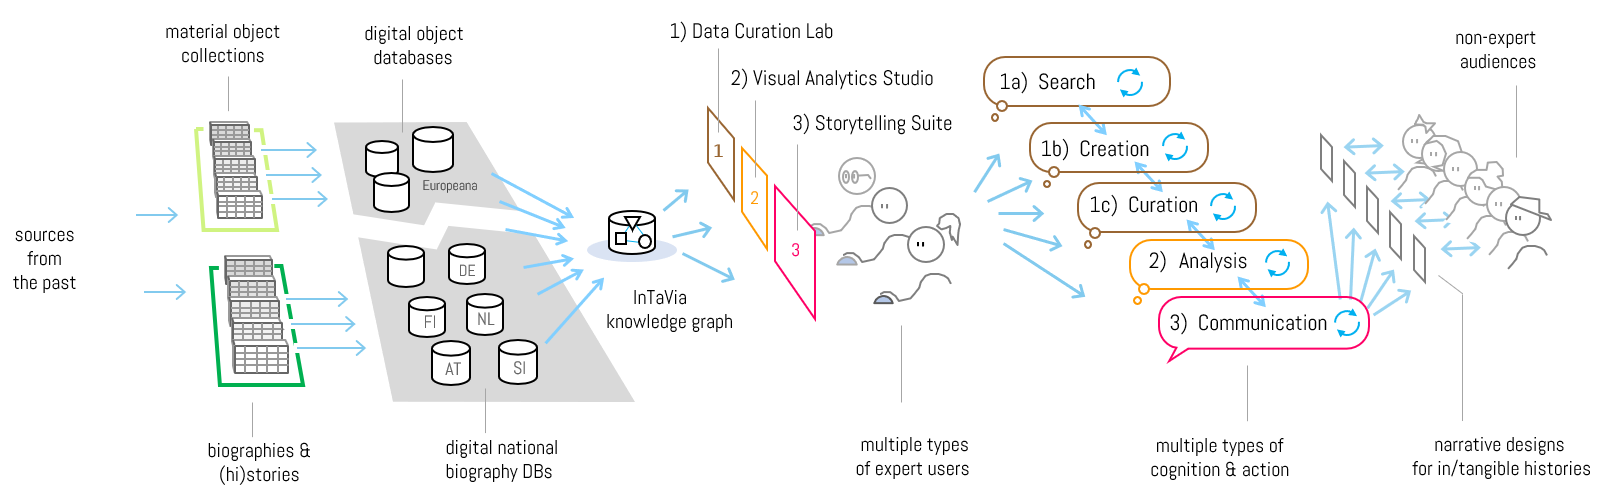
\includegraphics[width=0.8\textwidth]{images/image18.png}
	\caption{Architecture du projet}
	\label{fig:image18}
\end{figure}


\begin{center}
	Depuis : Liem, Kusnick, Beck, Windhager, Mayr \enquote{A workflow approach...}
\end{center}

L’interface d’\textit{InTaVia} (cf. images ci-après) concilie donc tous les usages : de l’utilisateur cherchant à connaitre une thématique particulière, au conservateur de musée souhaitant créer une exposition en ligne en passant par le chercheur souhaitant simplement consulter les collections agrégées. Il parvient donc à concilier la tension entre trouvabilité et découvrabilité.


\begin{figure}[h!]
	\centering
	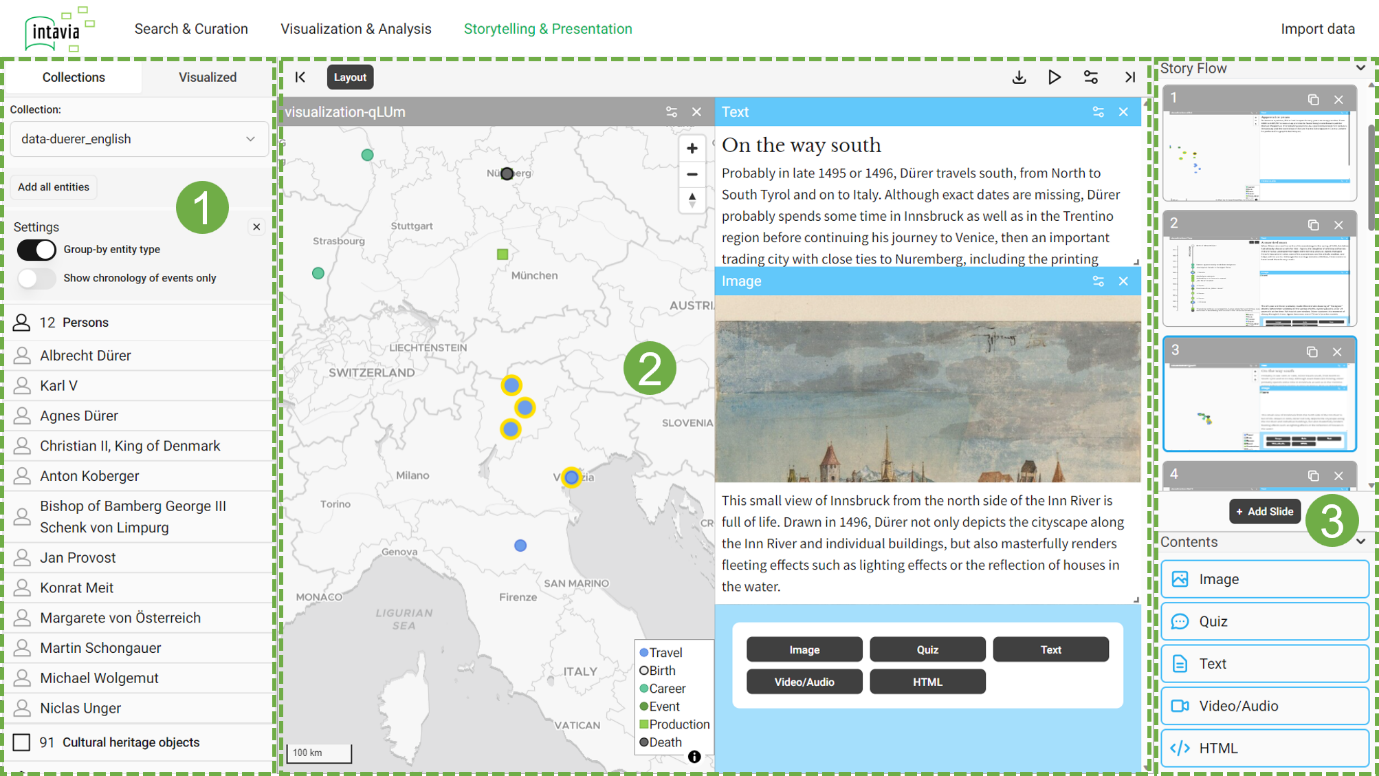
\includegraphics[width=0.8\textwidth]{images/image19.png}
	\caption{L’interface de création des histoires}
	\label{fig:image19}
\end{figure}
 
\begin{center}
	Depuis : Liem, Kusnick, Beck, Windhager, Mayr \enquote{A workflow approach...}
\end{center}




\begin{figure}[h!]
	\centering
	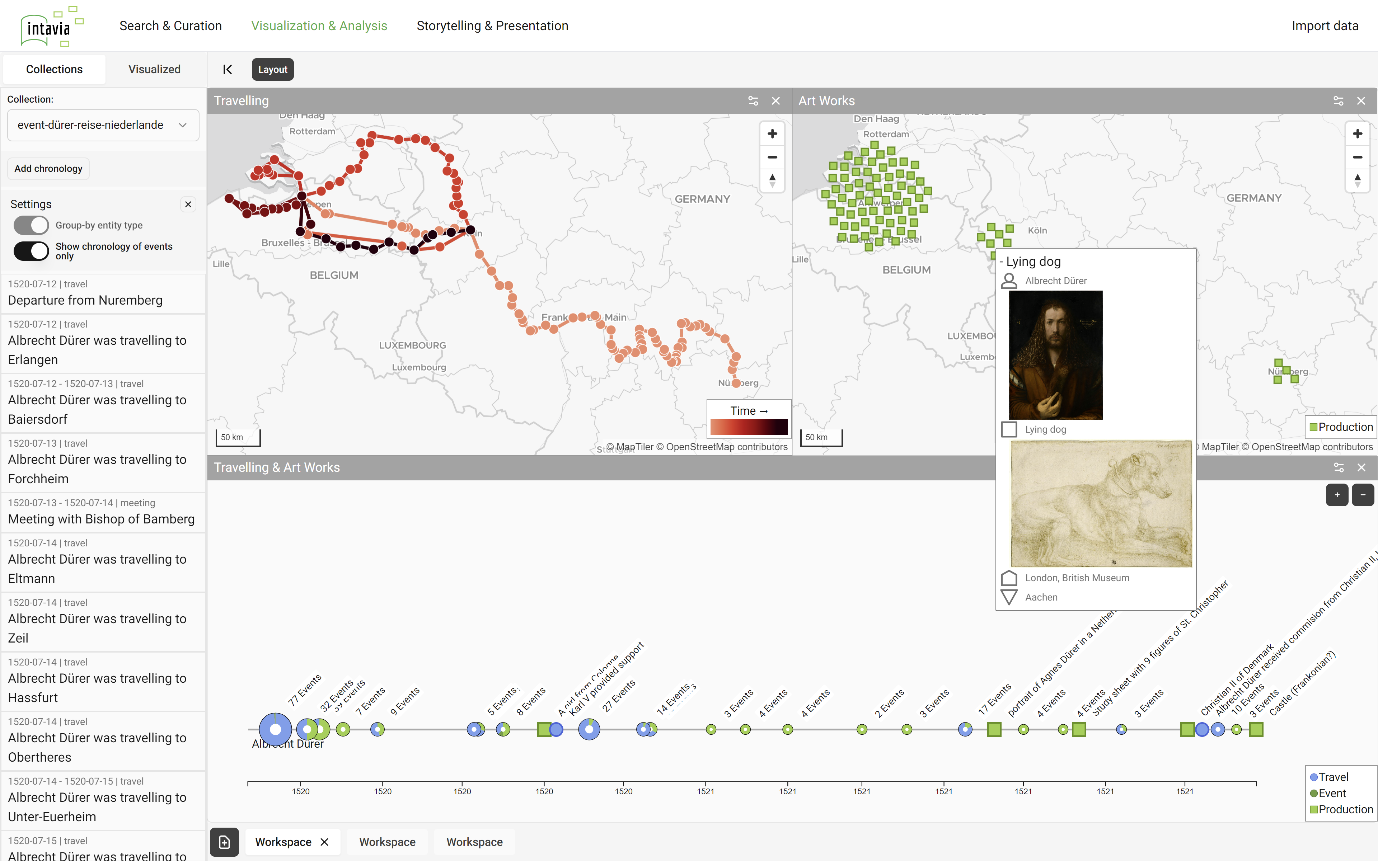
\includegraphics[width=0.8\textwidth]{images/image20.png}
	\caption{Exemple d'histoire créée (même source)}
	\label{fig:image20}
\end{figure}


\newpage

\subsection{Vers un nouveau \textit{crowdsourcing} reponsant sur l'ouverture des données}


« \enquote{Au Walters art museum, nous avons adopté cette approche [celle de l’\textit{open data}, N.D.A] et nous avons mis nos manuscrits sur le web pour que tout le monde puisse les voir, toutes les données brutes, toutes les descriptions, toutes les métadonnées, sous une licence \textit{“Creative commons”}. […] Et le résultat, c’est que si vous lancez une recherche d’images dans Google en tapant “Illuminated manuscript Koran”, par exemple, 24 des 28 images que vous obtiendrez viennent de mon institution}\footcite{noel_william_nodate}.

En avril 2012, William Noel, conservateur au Walter Art Museum, consacrait un \textit{TED talk} au \enquote{Codex Perdu d’Archimède en apparence}, mais en réalité, l’acmé de son intervention semble être le moment où il révèle que toutes les données du projet sont en accès libre. Et si l’on regarde la conférence avec cette clé de lecture en tête, on se rend compte qu’elle est parsemée de références à cette notion : des scribes médiévaux copiant les textes antiques, on passe facilement aux internautes créant leur propre collection et s’emparant du patrimoine numérisé. Pour William Noel, non seulement l’\textit{open data} est \enquote{un avantage pour l’humanité et ce genre de choses}, mais aussi pour les institutions \enquote{parlons de choses égoïstes}\footcite[à 13 minutes 26secondes]{noel_william_nodate}, selon lui : les gens vont au Louvre, car ils souhaitent y voir la Joconde, et ils veulent la voir, car ils la connaissent déjà, car ils ont déjà vu des milliers d’images de l’œuvre : parfois détournées (on pense à l’œuvre de Duchamp\footcite{zotero-368}, mais aussi de façon plus contemporaine aux \textit{memes}\footnote{Concept (texte, image, vidéo) massivement repris, décliné et détourné sur Internet de manière souvent parodique, qui se répand très vite - Larousse}). La constitution de \enquote{communs numériques}\footcite[p. 173]{bermes2024} revêt alors une importance capitale, non seulement dans la préservation, mais aussi dans la transmission\footcite[p. 175]{bermes2024} : permettre aux utilisateurs d’interagir avec le patrimoine (qui doit pour cela être ouvert) fait donc en sorte, entre autres choses, qu’il soit mieux repéré en ligne et plus visionné : car on est beaucoup plus enclin à suivre la recommandation de tiers de confiance (ici, d’autres internautes collaborant au projet) que celle d’une institution\footcite{ertzscheid2019}.

Si nous avons titré cette partie \enquote{vers un nouveau \textit{crowdsourcing}} c’est parce que nous avons observé que la participation en ligne des internautes avait évolué ces dernières années, si avant les activités principales se résumaient plus en un \textit{digital labor} : c’est-à-dire \enquote{la captation de la valeur générée par les activités des internautes en ligne}\footcite{zotero-365} avec des activités qu’Oomen et Aroyo classaient en six domaines en 2011\footcite[(cité par)]{neroulidis_crowdsourcing_2015} : correction/transcription, contextualisation, enrichissement, classification, co-curation et \textit{crowdfunding}. Désormais, les activités en ligne des internautes semblent se tourner vers la notion de communs numériques. On peut exemplifier ce propos avec le site \textit{notrehistoire.ch} lancé en 2009 par la Fonsart\footnote{Fondation pour la sauvegarde de la Radiotélévision, association créée en 2012 par la RTS} avec trois mots d’ordre : publier, participer et explorer\footcite{zotero-361}. Il propose à ses utilisateurs de participer à la création d’un patrimoine commun basé à la fois sur des archives institutionnelles et des archives personnelles. Il est structuré tel un réseau social en suivant les pratiques du \textit{web 2.0} où l’on peut commenter, créer, partager et publier du contenu en utilisant les archives disponibles sur le site provenant d’une part d’institutions romandes et de l’autre de particuliers.  

Le site est ainsi organisé comme un réseau social, où l’on voit des publications d’internautes défiler toujours avec la possibilité d’interagir, on peut aussi choisir d’aller explorer différentes thématiques, voir celles qui sont les plus alimentées, profiter du classement chronologique ou des différents \textit{tags} (identifiés par un dièse dans les publications des internautes) : bref, cela ressemble énormément à un réseau social classique.



\begin{figure}[h!]
	\centering
	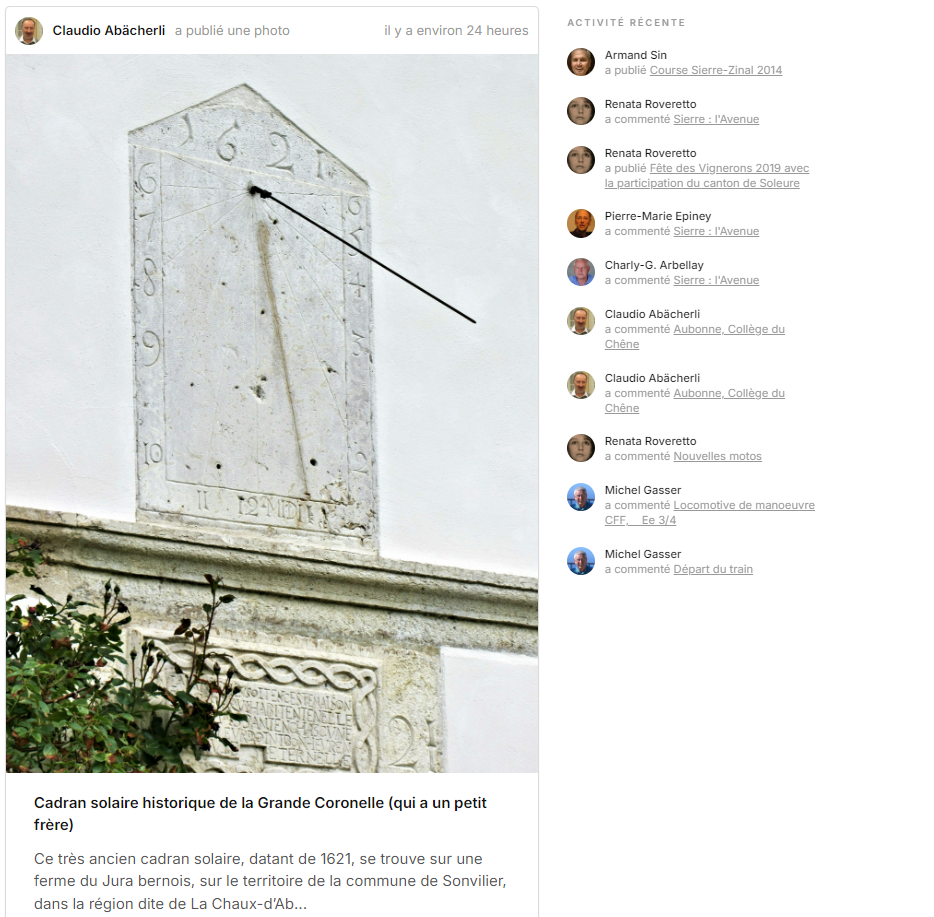
\includegraphics[width=0.8\textwidth]{images/image22.png}
	\caption{L'interface de notrehistoire.ch}
	\label{fig:image21}
\end{figure}

\begin{center}
	\url{https://notrehistoire.ch/feed}
\end{center}

Outre le fait qu’il brise les frontières : à la fois physiques entre des documents séparés et organisationnelles, il faut noter que les institutions perdent leur rôle de prescription et deviennent des contributrices à la constitution d’un Lieu de mémoire commun\footnote{Toujours en références aux ouvrages parrus sous la direction de Pierre Nora}. Comme Emmanuelle Bermès le rappelle dans son ouvrage : \enquote{leur nouveau défi [des institutions patrimoniales] est d’accompagner et de faciliter l’appropriation du patrimoine numérique par ses communautés bénéficiaires}\footcite[p. 186]{bermes2024}. Même si évidemment, les pratiques de \textit{crowdsourcing} plus classiques identifiées plus haut ne disparaissent pas, il semble que ce nouveau type de pratique, grâce à des interfaces renouvelées, prenne une place de plus en plus importante.


\subsection{L'intelligence artificielle comme porte d'accès au savoir, encore faut-il trouver la clé}

Précisons ici que nous ne nous concentrerons que sur un seul cas d’usage de l’intelligence artificielle ici, le \textit{RAG} (\textit{retrieval augmented generation}/génération augmentée de récupération), car il nous semble le plus proche de notre sujet de découvrabilité dans le secteur patrimonial. Par ailleurs, nous avons déjà abordé un autre champ d’application de l’intelligence artificielle dans ce mémoire en parlant d’algorithmes de recommandation.

Comme pour ces derniers, une explication technique est indispensable pour cerner les enjeux autour de cette technologie. Un \textit{RAG} est un grand modèle de langue (le plus connu étant \textit{chat GPT}) qui, pour répondre à une question de l’utilisateur (on parle de \textit{prompt}), utilise des données fournies préalablement en tant que source\footcite{pouyllau_quels_2024}. Cette approche combine donc les extraordinaires possibilités des modèles de langues dans la génération de réponses tout en corrigeant leur principal défaut : le manque d’indication des sources et le phénomène d’hallucination\footnote{Dans le domaine de l'intelligence artificielle, une hallucination ou une confabulation est une réponse fausse ou trompeuse qui est présentée comme un fait certain ; par exemple, un chatbot qui génère un chiffre d'affaires pour une entreprise sans avoir de données à ce sujet. - Wikipédia} ; en bref, leur manque de fiabilité. Pour les fonds patrimoniaux et leur découvrabilité, le potentiel d’une telle technologie est prometteur. Cela améliorerait grandement la recherchabilité en permettant aux utilisateurs de saisir, en langage naturel, leurs requêtes. De l’ère des équations de recherche, nous étions passés aux requêtes \textit{Google-like} avec le \textit{RAG}, nous passerions à l’ère du questionnement en langage naturel\footcite{bermes_futur_2024}. Car le changement de paradigme principal de l’intelligence artificielle dite générative est bien celui-là : ce ne sont plus les humains qui font l’effort de communiquer dans une langue adaptée aux ordinateurs, mais le contraire, ce qui marquerait un « passage de la communication homme-machine à la communication machine-homme »\footcite[p. 7]{pillaud_et_2024}. En termes de découvrabilité, cela signifierait qu’un chercheur/utilisateur du fonds de la RTS (par exemple) pourrait directement demander dans une interface (souvent un \textit{chatbot} dans le cas du \textit{RAG}) « tous les documents concernant l’histoire de la Radiodiffusion en Suisse » dans le fonds de la RTS, ce qui évidemment — outre le fait d’être un immense gain de temps — représente une perspective de recherchabilité incroyable, car une telle requête actuellement ne donnerait que peu de résultats, car ce champ n’existe pas dans le thésaurus.


\begin{figure}[h!]
	\centering
	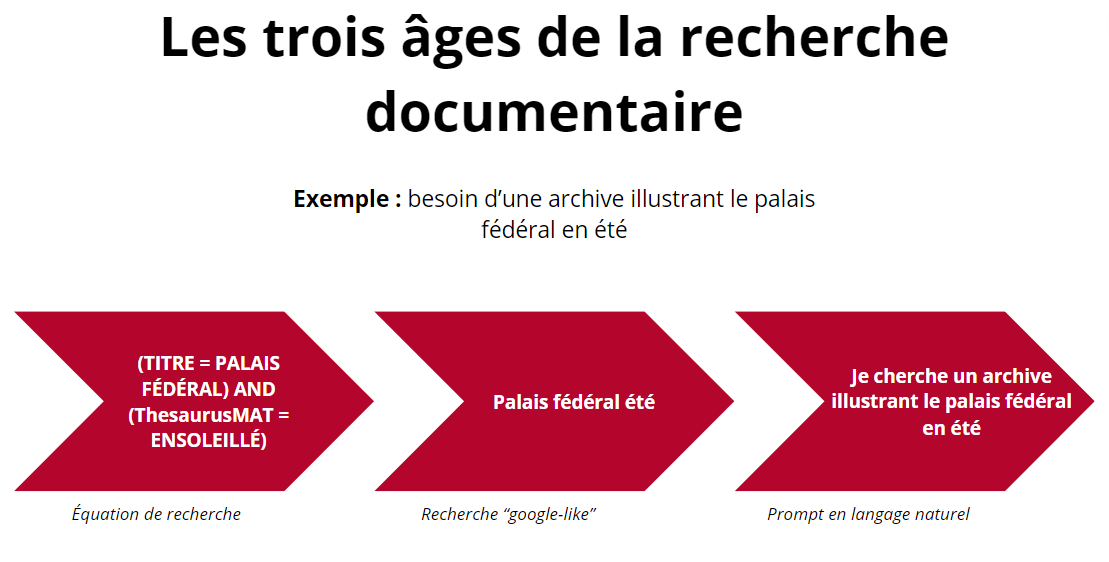
\includegraphics[width=0.8\textwidth]{images/image23.png}
	\caption{Illustration réalisée par nos soins.}
	\label{fig:image23}
\end{figure}

Si la mise en place de \textit{RAG} peut être vue comme une perspective passionnante pour les acteurs patrimoniaux, il n’en reste pas moins que cela pose de nombreux défis. Défi écologique d’abord (nous le détaillerons dans notre partie 3). Défi éthique et juridique ensuite, la mise en place d’un \textit{RAG} nécessite d’utiliser un grand modèle de langue (que les institutions patrimoniales ne développeront jamais en interne) provenant de sociétés privées : Google ou \textit{Open AI} notamment, qui est ensuite adapté (« \textit{fine tuné} ») avec les données internes pour être utilisé. Mais pour faire cela, il faut envoyer les données aux serveurs des entreprises (par le biais d’interfaces de programmation ou \textit{API}), car il est très difficile d’entrainer localement ces modèles qui ont besoin d’une infrastructure importante et ne sont pas \textit{open source}. Même si depuis peu \textit{Open AI} et Google ont indiqué ne pas utiliser les données transférées pour entrainer leurs modèles\footcite{rochefort2023}, ces dernières sont tout de même stockées sur leurs infrastructures ce qui pose des questions de gouvernance de la donnée et de confidentialité en cas d’attaque.

Notons d’ailleurs que pour ces sociétés, les données extrêmement bien structurées des institutions patrimoniales sont véritablement du pain béni, en témoigne le récent partenariat qu’un consortium de trois sociétés spécialisées dans l’intelligence artificielle générative (\textit{Mistral AI}, \textit{Giskard} et \textit{Artefact}) ont tissé avec la Bibliothèque nationale de France et l’Institut national de l’audiovisuel français\footcite{clavey_bnf_2024}. La BnF précise d’ailleurs : « le monde a redécouvert que toutes les bibliothèques nationales comme la BnF sont des grands réservoirs de données. Le nôtre est probablement le plus grand réservoir de données propres et qualifiées au monde. D’un seul coup, ça intéresse donc nos petits camarades qui travaillent sur l’intelligence artificielle parce qu’au-delà du logiciel, il faut de la donnée pour les entrainer ». Ces « grands réservoirs » deviendront sûrement un enjeu très important dans les années à venir puisque les besoins en données de l’intelligence artificielle générative sont de plus en plus importants. Les chercheurs évoquent d’ailleurs la date de 2026 comme celle où toutes les données publiques de l’Internet auront été aspirées par les modèles en formation\footcite{forbes_internet_2024}. Même si beaucoup évoquent la possibilité de former ces modèles par des contenus générés par intelligence artificielle, il semble que cette piste ne donne pas de résultats très probants (pour l’instant, le domaine étant en évolution constante)\footcite{noauthor_entrainer_nodate}.

Il y a, enfin, un défi de repérabilité, ces technologies ne font pas de miracles : si une partie du fonds n’a que peu de métadonnées, elle ne sera pas renvoyée. Prenons l’exemple de la RTS ici, on a noté dans notre état des fonds que le sport et les émissions pour enfants ont été peu archivés, et quand c’est le cas avec des métadonnées minimales : si un \textit{RAG} est mis en place, ces collections resteront invisibilisées, car mal documentées et en petit nombre. L’exemple de Robert Williams est ici tristement éclairant. En 2020, ce dernier, afro-américain, a été arrêté et a passé trente heures en détention parce qu’un logiciel d’intelligence artificielle avait confondu sa photographie avec celle d’un voleur de montre\footcite{noauthor_etats-unis_nodate}. Ce que cela vient prouver, c’est que les algorithmes, conçus en grande partie par des blancs, commettent bien plus d’erreurs sur des groupes ethniques moins représentés dans leurs données d’entrainement que ceux majoritaires. (Il y a ici un enjeu d’explicabilité algorithmique que nous traiterons aussi dans notre partie 3).

Au regard de ce qui a été écrit, il est essentiel, avant de se lancer dans la mise en production de \textit{RAG} pour des collections patrimoniales, de réaliser un travail en profondeur sur les données et leur pondération. Dans le cas de la RTS, cela passerait par une transcription automatique de tous les programmes et la génération de résumés documentaires pour chacun (en utilisant comme données d’entrainement ceux déjà rédigés) ainsi que de mots-clés documentaires issus des thésaurus. Cela permettra un entrainement plus efficace (avec des coûts environnementaux et financiers réduits), car nécessitant moins d’itérations tout en réduisant les biais d’invisibilisation décrits, car tous les documents seront documentés avec la même précision.

Concluons avec ce qu’écrit Emmanuelle Bermès dans un article de blog : « si ce genre de méthode doit révolutionner à terme la recherche documentaire et voir nos recherches par mots-clés disparaître au profit de \textit{prompts}, comme la recherche par équation a disparu au profit de la recherche plein texte… On a intérêt à comprendre comment elles fonctionnent et à apprendre à les maitriser. Car le \textit{prompting}, c’est comme la recherche documentaire : ça pourrait paraître simple à première vue, mais c’est une compétence de la littératie numérique qui ne s’invente pas\footcite{bermes_futur_2024}.

